%CS4099 Dissetation
%!TEX root = ../Project.tex
\section{Design}
\subsection{Tilemap}

There were two main choices for the isometric tilemap, a `Diamond' map or a  `Staggered' map \cite{isometric_game_programming}, examples of both are shown below.

\def\tilemapSize{5in}
\begin{figure}[htbp]
	\begin{center}

	\subfigure[Diamond Map]{
		\label{fig:tilemap1} 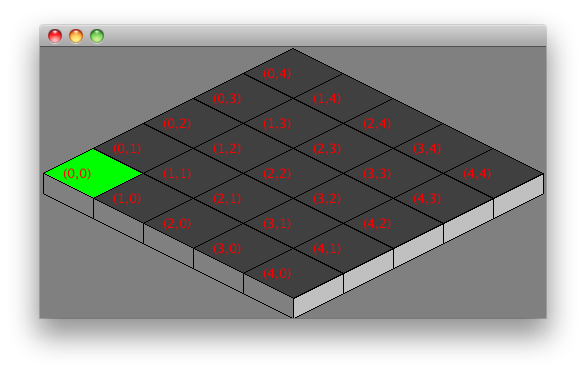
\includegraphics[width=\tilemapSize]{figures/tilemap1.png}} 
	\subfigure[Staggered Map]{
		\label{fig:tilemap2} 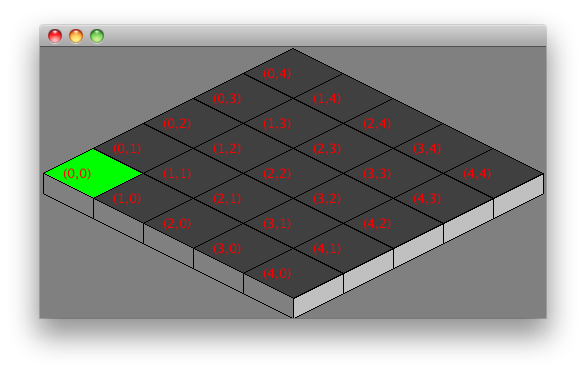
\includegraphics[width=\tilemapSize]{figures/tilemap2.png}} 
	\caption{\label{fig:tilemap0} The two main types of isometric tilemaps}
	\end{center}
\end{figure}

The `Staggered' Map has following advantages:
\begin{itemize}
	\item The map fill up the screen with very little wasted space, so the user can more of what happing on the map.
\end{itemize} 

The `Diamond' map was chosen for the following reasons:
\begin{itemize}
	\item `Diamond' map look nicer then `Staggered' maps because they have no ragged edges.
	\item Since that maps are large (at lest 15 \* 15) the space wasted at the edges of the map does not matter as much.
	% TODO Check deegres (45?)
	\item Simpler to think about, since a `Diamond' map is just a rectangular map rotated by 45$^{\circ}$
\end{itemize}

\underline{Maths about isometric tilemaps? }